\subsection{Lazo de corriente} \label{sec:lazoI}

Se realizó la modificación de los parámetros nombrados en la sección \ref{sec:error} y se corroboró que el error no aparecía nuevamente al cambiar el modo de funcionamiento del variador.

Para realizar la comunicación del microcontrolador con el variador de velocidad se decidió utilizar el modo de funcionamiento de entrada analógica de dos hilos (\textbf{Ai1}: hilo de señal + hilo común) ingresados por la bornera de la figura \ref{fig:born}. Este modo analógico podía ser configurado de 0-10V o 0-20mA a través del “jummper J3” (Figura \ref{fig:placals}).

Se optó por la utilización del lazo de corriente, este tiene ventajas sobre el lazo de tensión ya  que es más estable en largas distancias y más inmune a los ruidos eléctricos e interferencias electromagnéticas respecto al lazo de tensión. Normalmente, se utilizan lazos de corriente de 4-20mA para poder observar si hubiera fallas en el circuito, por lo que fue necesario adaptar la señal generada por el $\mu$C para seguir el estándar.



\begin{figure}[h]
	\centering
	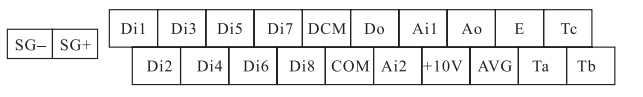
\includegraphics[width=0.7\linewidth]{imagenes/terminales.png}
	\caption{Terminales de control}
	\label{fig:born}
\end{figure}

\begin{figure}[htbp]
	\centering
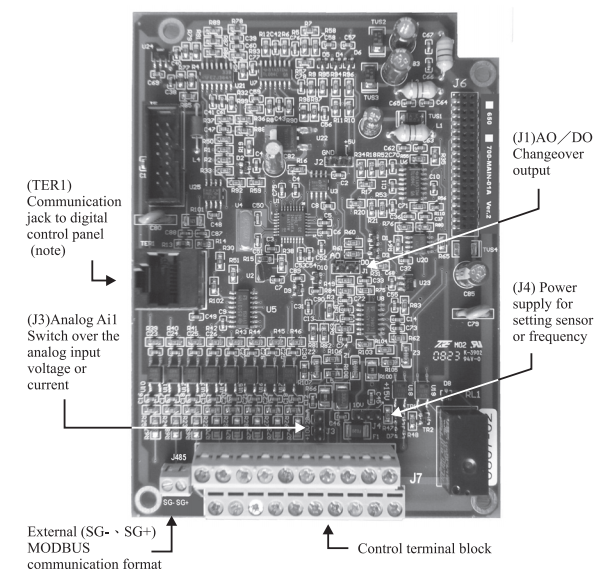
\includegraphics[width=0.7\linewidth]{imagenes/placa_ls}
\caption{Placa electrónica del variador de velocidad}
\label{fig:placals}
\end{figure}

La señal analógica para realizar el control del variador de velocidad fue generada por una señal PWM estipulada a través de la biblioteca \textit{TIMEROne} del microcontrolador. La instrucción \textit{Timer1.inizialize(period)} de la biblioteca Arduino inicializa el \textit{timer} con el valor de \textit{period}, este valor es el tiempo en el que se dispara el temporizador y en el caso de este proyecto es de 40 $u$s.

El otro comando que se utilizó fue \textit{Timer1.pwm(pin, duty)} que establece el número de
pin dónde sale la señal generada, en este caso pin 9 y \textit{duty} es un valor entre 0 y 1023 establecido por la programación. La salida del pin 9 corresponde a valores de tensión (de 0 a 5V), por lo que fue necesario realizar la transformación de esta señal a una señal de corriente a través una “placa adaptadora de señal” (Figura \ref{fig:adapt}). Esta placa, tiene como entrada el valor de tensión anteriormente nombrado y genera una señal de salida de 0 a 20mA; por medio de un parámetro del variador, esto modificó la señal para adaptarla al estándar de 4 a 20mA.

\begin{figure}[htbp]
	\centering
	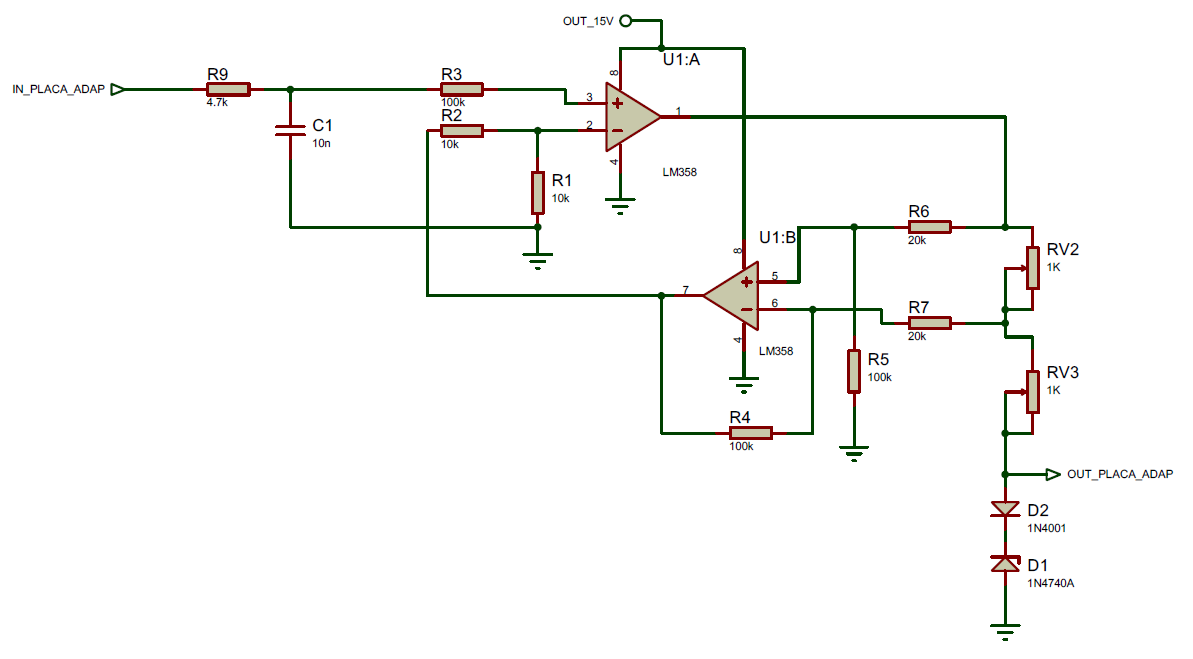
\includegraphics[scale=0.5]{adap_pl.png}
	\caption{Placa adaptadora de señal}
	\label{fig:adapt}
\end{figure}



\subsection{Estimación de la planta} \label{sec:estima}
    \subsubsection{Diagrama de trabajo}

Para realizar la estimación de la planta se muestra un diagrama de bloques del procedimiento que se siguió de forma resumida.

\begin{figure}[htb]
	\centering
	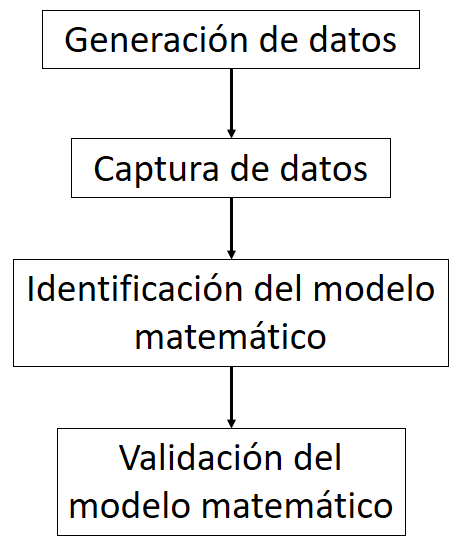
\includegraphics[scale=0.4]{planta_d.png}
	\captionof{figure}{Diagrama de bloques del procedimiento de modelado de la planta}
	\label{fig:planta_d}
\end{figure}

 \textbf{Generación de datos:} De acuerdo a diversas pruebas realizadas, se eligen las variables de mayor interés para analizarlas y asi poder enviar la información de forma eficaz.

 \textbf{Captura de datos:} A través del puerto serie y con Processing se realiza el almacenamiento de los datos de respuesta del sistema ante el estímulo de las señales de excitación. Posteriormente, el análisis de los datos y la generación de las gráficas correspondientes es realizado por medio de rutinas de código implementadas en Matlab.

 \textbf{Identificación del modelo matemático:} Se utilizaron varios métodos de identificación experimental, todos ellos analizados con la respuesta al escalón del sistema.

 \textbf{Validación del modelo matemático:} Una vez obtenida la mejor estimación, se efectuó una validación adicional a partir de la comparación de datos experimentales con los teóricos generados en simulaciones.






    \subsubsection{Método de estimación}

    Una vez que se determinó el valor de la ventana del filtro, velocidad de conmutación de PWM, tiempos de aceleración y desaceleración, etc, se utilizó el modo de ingreso de señal por lazo de corriente al variador de velocidad. 
    
    La Figura \ref{fig:bloques} muestra un diagrama resumido de los pasos a realizar para tomar datos de la planta. G(s) es el conjunto del túnel de viento, variador de velocidad y motor.


\begin{figure}[htbp]
	\centering
	\subfigure[Diagrama en bloques]{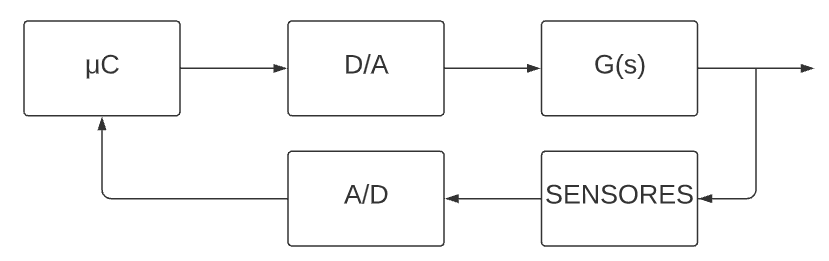
\includegraphics[scale=0.5]{bloques.png}}
	\centering
	\subfigure[Diagrama de conexión ]{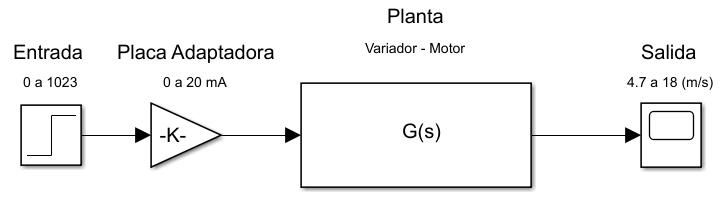
\includegraphics[scale=0.7]{Estimacion_1.png}} 
	\caption{Estimación de planta} \label{fig:bloques}
\end{figure}
 
    
    Para realizar la estimación de la planta se obtuvo y guardó tablas de datos con Processing, en las que se generó distintos escalones de entrada para la obtención de varias mediciones. En la figura \ref{fig:est2} se observa los valores de velocidad y los escalones que se realizaron durante una prueba generada para obtener los parámetros necesarios para la estimación de la planta.
    
    \begin{figure}[htb]
    	\centering
    	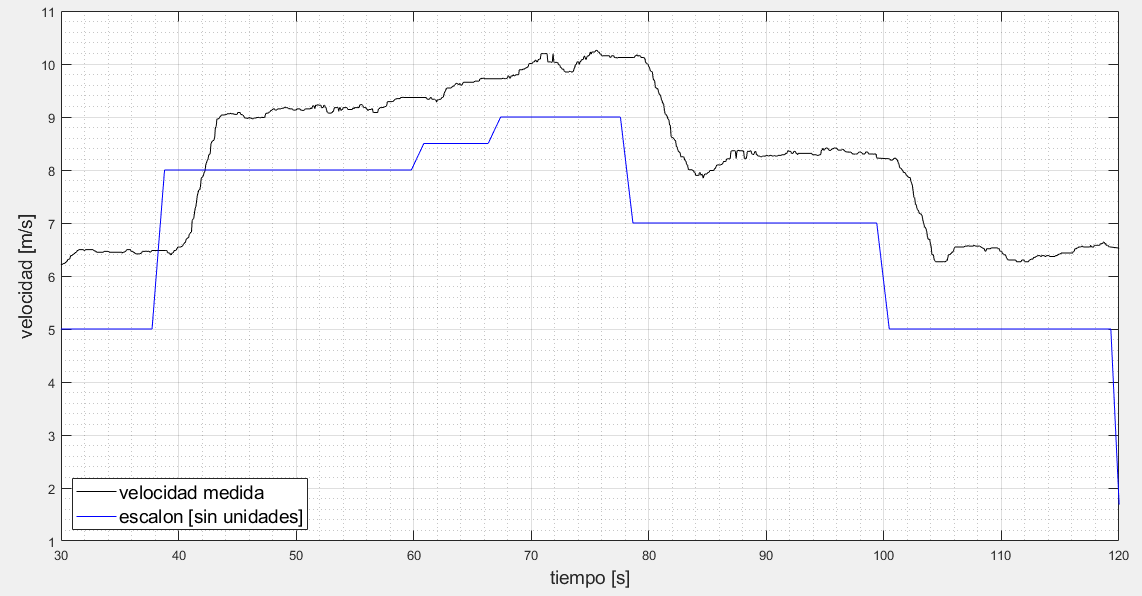
\includegraphics[scale=0.45]{estima.png} %pruba_1 del 0607
    	\captionof{figure}{Mediciones de velocidad a partir de distintos escalones dados}
    	\label{fig:est2}    
    \end{figure}
    
    Seguidamente, se procedió a generar un nuevo código de Matlab donde se cargó los datos obtenidos de la prueba (Figura \ref{fig:est2}) y con ellos se observaron las características necesarias de la figura (a) \ref{fig:pl2} para realizar la estimación de la planta a través de la comparación con la función de transferencia de un sistema de \textit{"2° orden con retardo"} \cite{pomares2011sistemas}.
    
    \begin{figure}[H]
    	\centering
    	\subfigure[Parámetros respuesta 2° orden]{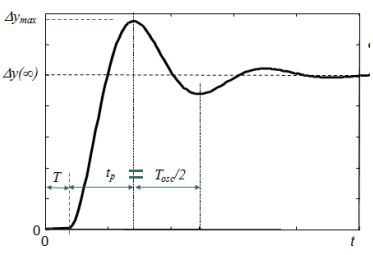
\includegraphics[scale=0.7]{parametros_seg.png}}
    	\subfigure[Estimación de parámetros]{\includegraphics[scale=0.45]{planta_seg1.png}} 
    	\caption{Estimación de planta} \label{fig:pl2}
    \end{figure}

El sistema de \textit{"2° orden con retardo"} posee la función de transferencia observada en la ecuación \ref{ec:G}.

 \begin{equation}
 	G(s)=\frac{k\omega_n^2}{s^2+2\xi\omega_ns+\omega_n^2}\ast e^{-T.s}
 	\label{ec:G}
 \end{equation}

La ecuación de sobre oscilación (Ecuación \ref{ec:amort}), es utilizada para calcular el factor de amortiguamiento ($\xi$)
\begin{equation}
	\delta\;=\;\frac{\triangle y_{max}-\triangle y\left(\infty\right)}{\triangle y\left(\infty\right)}=\;e\;^{-\frac{\xi\pi}{\sqrt{1-\xi^2}}}
	\label{ec:amort}
\end{equation}

La ecuación \ref{ec:tp} es utilizada para obtener el valor de la frecuencia natural ($\omega_n$) a partir del tiempo de pico.
\begin{equation}
t_p\;=\;\frac{T_{osc}}2\;=\;\frac\pi{\omega_n\sqrt{1-\xi^2}}
\label{ec:tp}
\end{equation}

    
    Con ayuda de un código generado en Matlab y ajustes manuales se llegó a la siguiente función de transferencia de segundo orden:
    
    \begin{equation}
    	\frac{Y(s)}{U(s)}=\frac{0,02483}{s^2+1,846s+1,535}*e^{-1.2.s}
    \end{equation}
   
    Esta función de transferencia se realizó para una entrada entre 0 y 1023, los cuales son el límite mínimo y máximo para determinar el ancho de pulso de la señal PWM del $\mu$C como se ve en la sección \ref{sec:lazoI}.
    
    Para corroborar la elección de la planta se realizó en \textit{Simulink} la respuesta del sistema a los mismos escalones experimentales. En la figura \ref{fig:estim2} y \ref{fig:estim3}, se dispuso la respuesta experimental y la simulada para realizar la comparación.
    
    \begin{figure}[H]
    	\centering
    	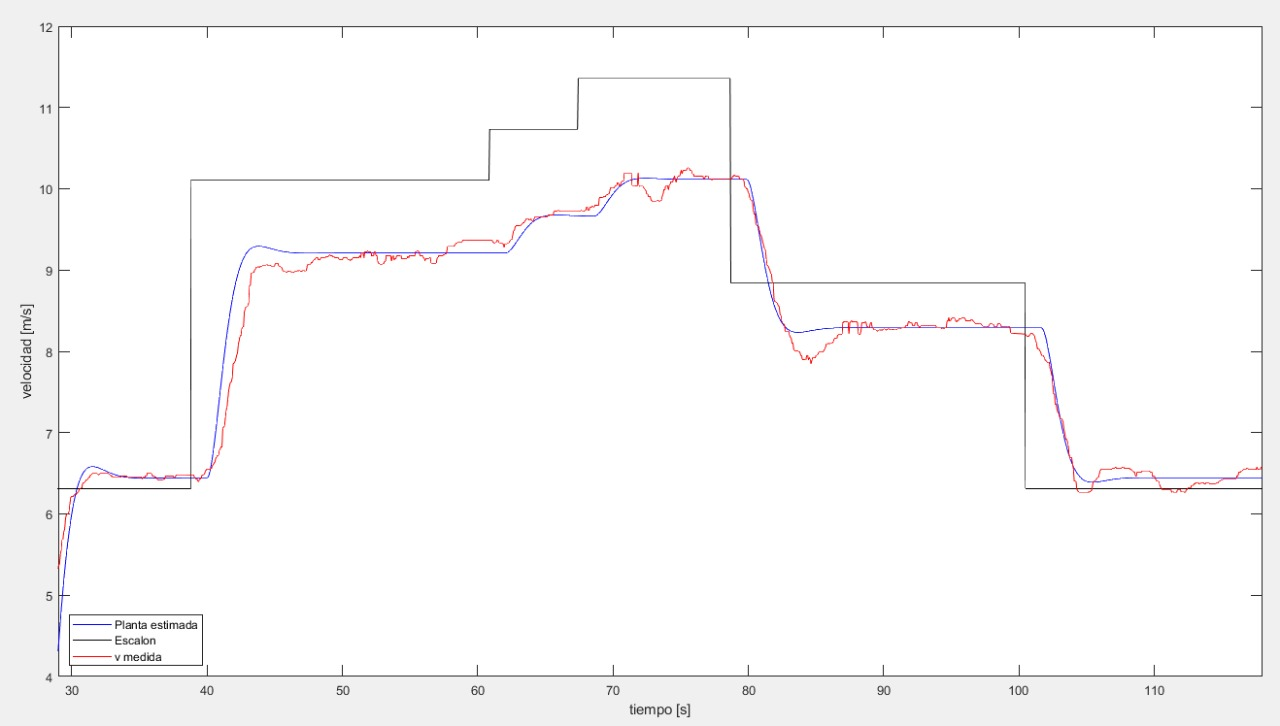
\includegraphics[scale=0.3]{estim2.jpeg}
    	\captionof{figure}{Corroboración de estimación de la planta. Ejemplo 1}
    	\label{fig:estim2}
    \end{figure}

\begin{figure}[H]
	\centering
	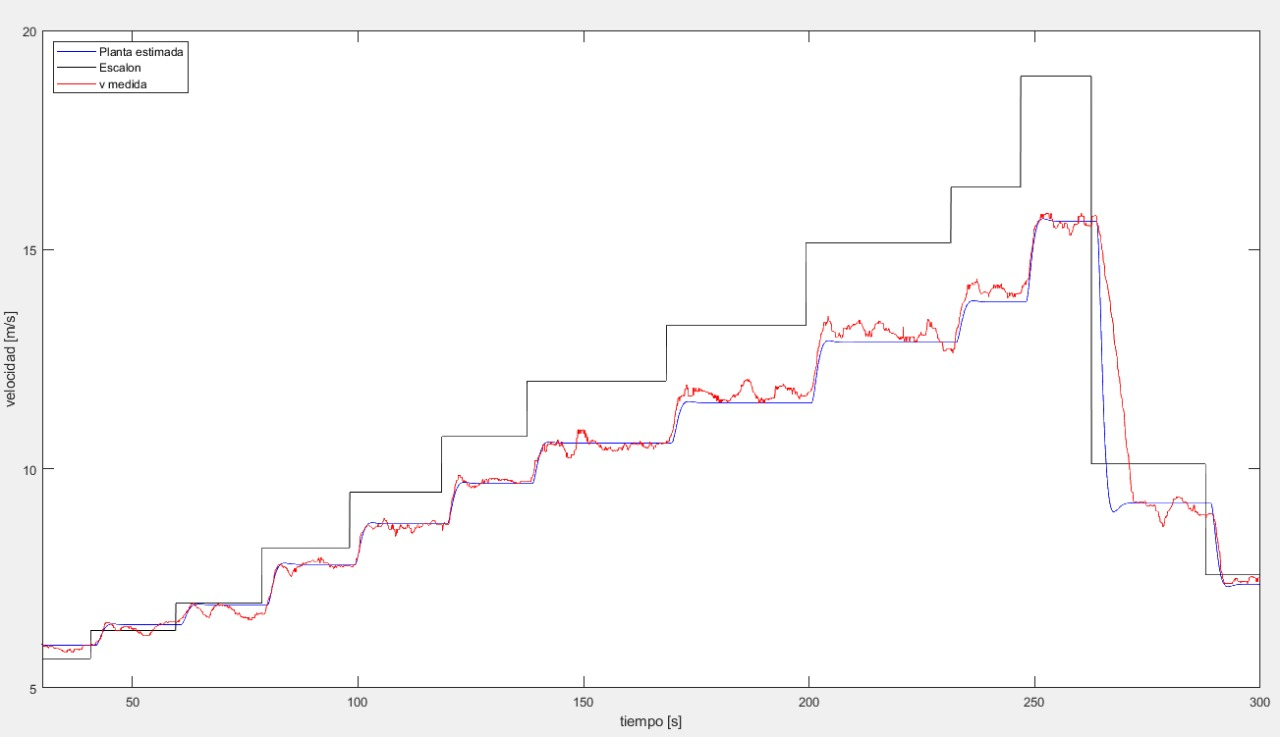
\includegraphics[scale=0.3]{estim3.jpeg}
	\captionof{figure}{Corroboración de estimación de la planta. Ejemplo 2}
	\label{fig:estim3}
\end{figure}
       
    \subsection{Control}
    Para el cálculo en primera instancia del controlador PID, se utilizó la herramienta de \textit{Matlab}, y a partir de los primeros valores se realizaron pequeñas modificaciones, todas con el formato PI (proporcional - integrador) hasta obtener varios tipos de respuesta.
    Con los distintos valores de PI (Tabla \ref{tab:pid}) se realizaron pruebas en el Túnel del viento con escalones en la velocidad de referencia de 6 - 7,5 - 8,5 - 7,5 - 7 - 6 m/s,  un total de 5 ensayos para los mismos estímulos de entrada. En la figura \ref{fig:Lazo_Control} se observa el lazo de control que se utilizó. 
   
    \begin{figure}[H]
   	\centering
   	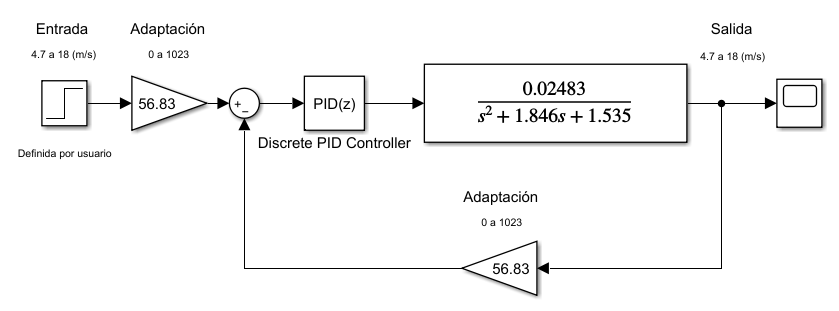
\includegraphics[scale=0.7]{Lazo_Control1.png}
   	\captionof{figure}{Lazo de control}
   	\label{fig:Lazo_Control}
   \end{figure}
    \begin{figure}[H]
    	\centering
    	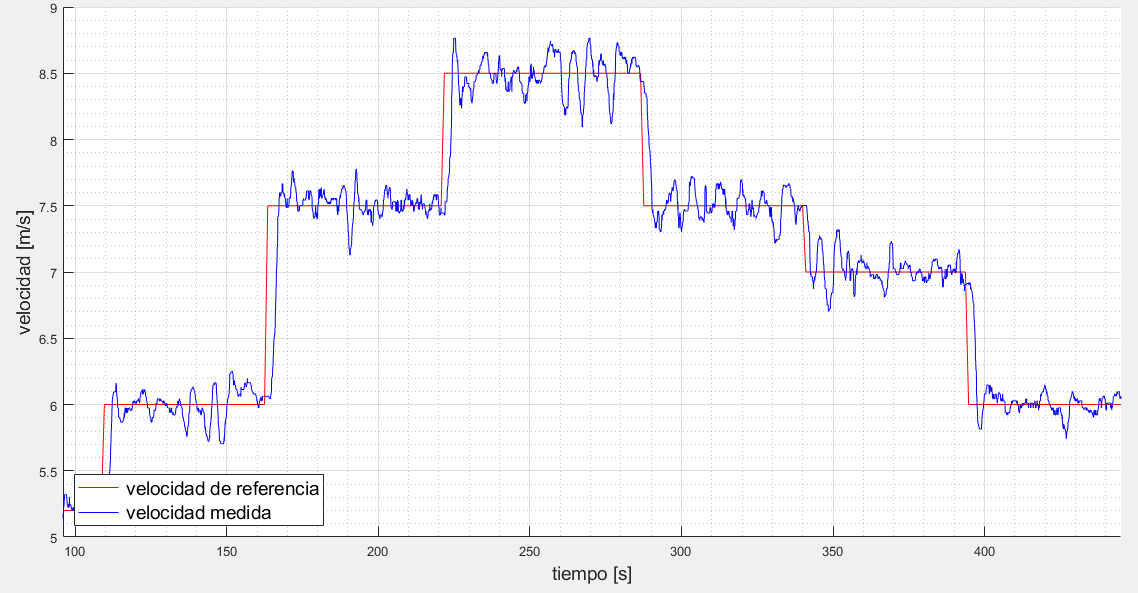
\includegraphics[scale=0.5]{pruebapid.png}
    	\captionof{figure}{Ejemplo de prueba realizada}
    	\label{fig:PI3}
    \end{figure}
    
    Los valores de cada configuración PI se muestran en la tabla siguiente
    \begin{table}[H]
    	\centering
    	\begin{tabular}{r|r|r|r|r|r|r|}
    		\cline{2-7}
    		\multicolumn{1}{l|}{} & \multicolumn{1}{c|}{\textbf{PI anterior}} & \multicolumn{1}{c|}{\textbf{Prueba3}} & \multicolumn{1}{c|}{\textbf{Prueba4}} & \multicolumn{1}{c|}{\textbf{Prueba5}} & \multicolumn{1}{c|}{\textbf{Prueba6}} & \multicolumn{1}{c|}{\textbf{Prueba7}} \\ \hline
    		\multicolumn{1}{|r|}{\textbf{P=}} & 0.225 & 0.0699 & 0.244 & 0.5451 & 0.6846 & 0.3286 \\ \hline
    		\multicolumn{1}{|r|}{\textbf{I=}} & 0.326 & 0.2035 & 0.2756 & 0.3599 & 0.4183 & 0.3107 \\ \hline
    	\end{tabular}
    \caption{Valores de PID's}
    \label{tab:pid}
    \end{table}
    
    Al visualizar las respuestas obtenidas por las diferentes configuraciones se puede realizar la comparación para un escalón en donde la velocidad sube (figura \ref{fig:pisubuda}) y otro donde la velocidad baja (figura \ref{fig:pibajada}).
    
    \begin{figure}[H]
    	\centering
    	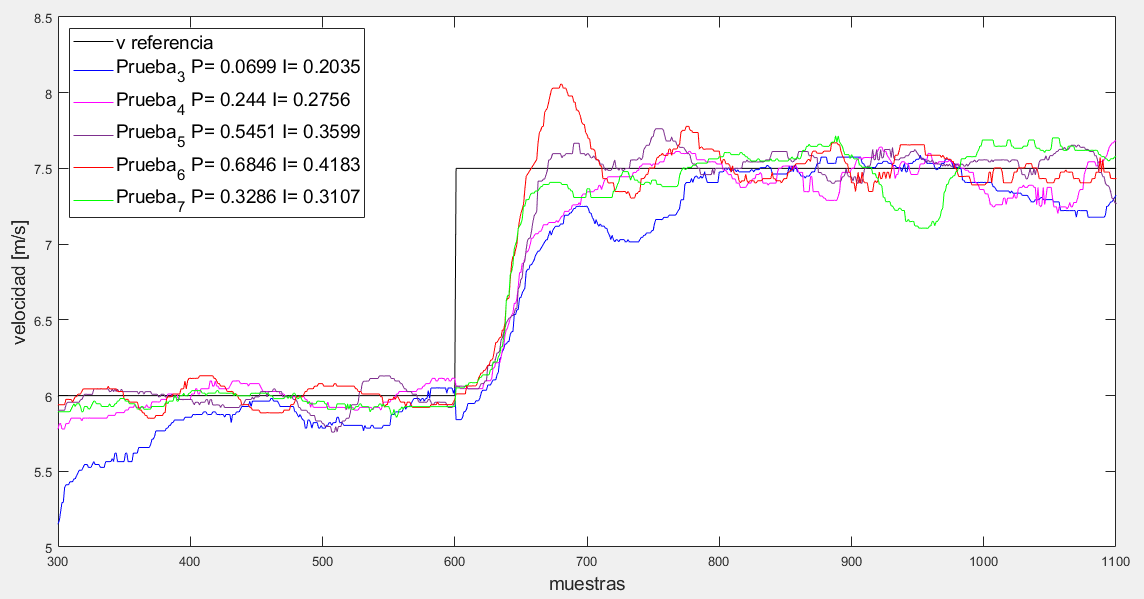
\includegraphics[scale=0.5]{pisubida.png}
    	\captionof{figure}{Comparación de PI, escalon de subida}
    	\label{fig:pisubuda}
    \end{figure}
    
    \begin{figure}[H]
    	\centering
    	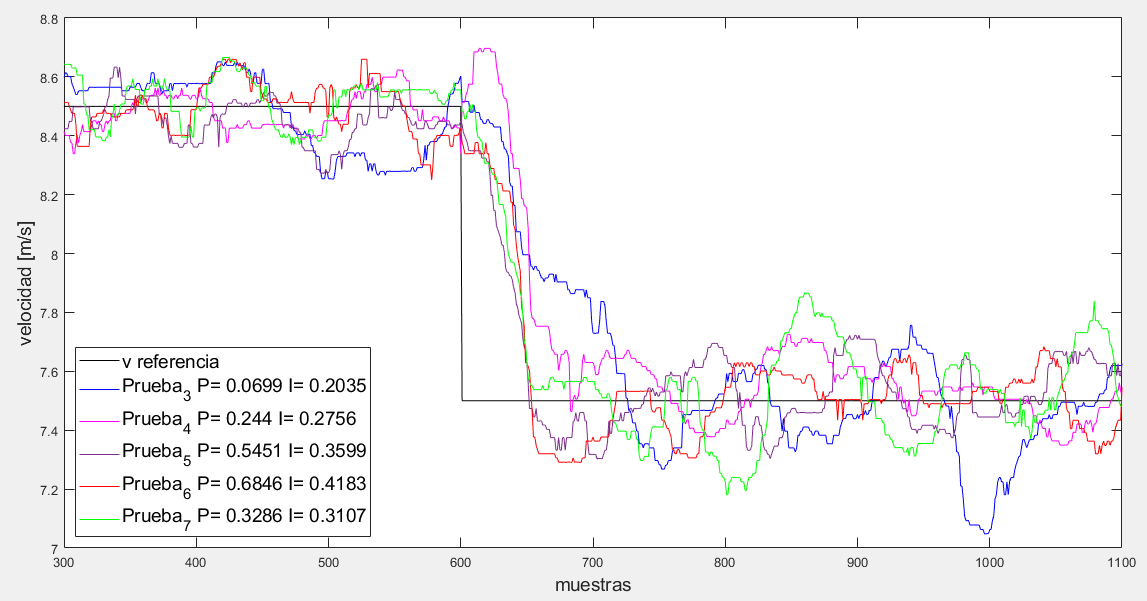
\includegraphics[scale=0.5]{pibajada.png}
    	\captionof{figure}{Comparación de PI, escalon de bajada}
    	\label{fig:pibajada}
    \end{figure}
    
    
    En la figura \ref{fig:mix} se pueden observar el sistema que genera mayor sobrepico, un sistema con una respuesta mas lenta, y un sistema con respuesta intermedia. 
    \begin{figure}[H]
    	\centering
    	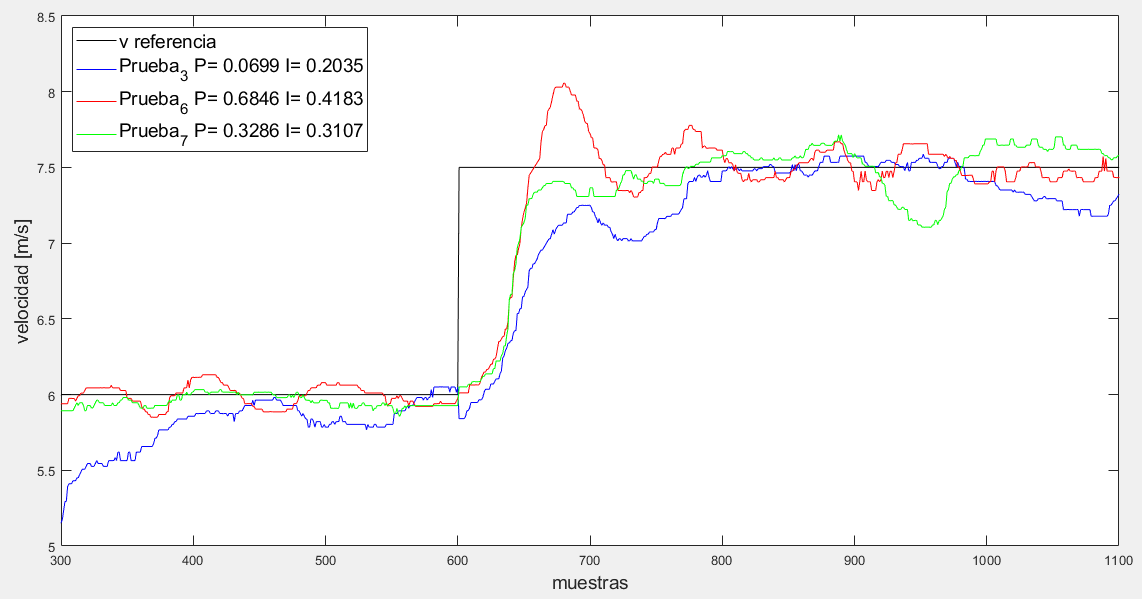
\includegraphics[scale=0.5]{mix.png}
    	\captionof{figure}{Comparación 3 sistemas PI}
    	\label{fig:mix}
    \end{figure}

	Al analizar los ensayos y obtener respuestas del sistema parecidas a las generadas en simulación, se determinó que la estimación de la planta se realizó de manera correcta, esto añadió mayor validez al sistema de simulación empleado en todas las pruebas. 
	
	\begin{figure}[H]
		\centering
		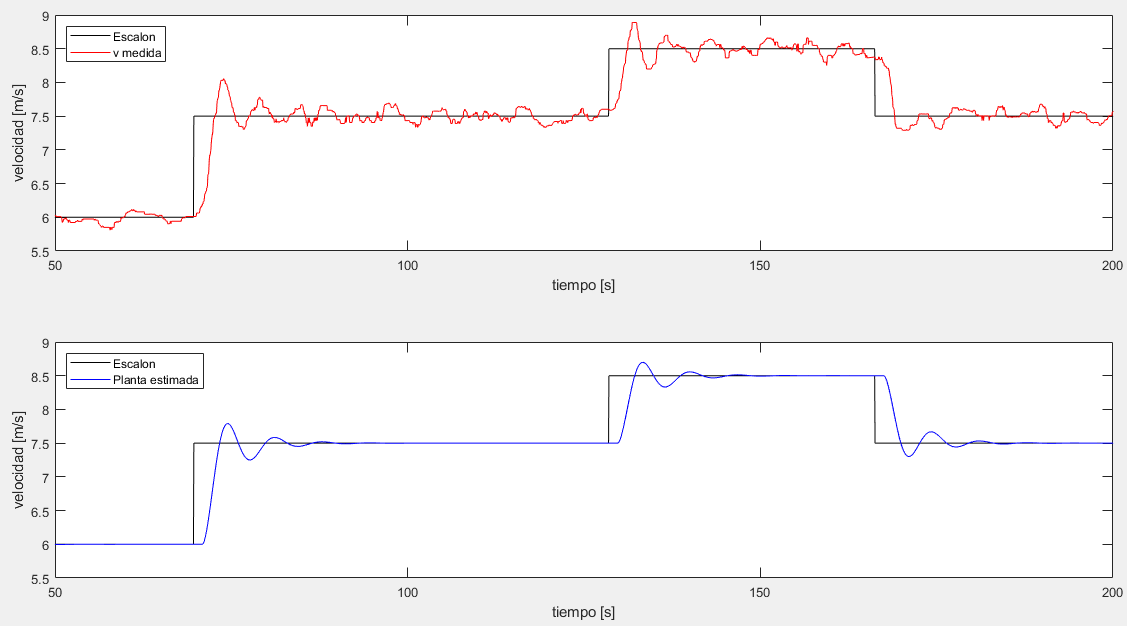
\includegraphics[scale=0.5]{Compa_Prueba6.png}
		\captionof{figure}{Datos Experimentales y Simulados para la \textit{Prueba6}}
		\label{fig:Prueba_6}
	\end{figure}   
\begin{figure}[H]
	\centering
	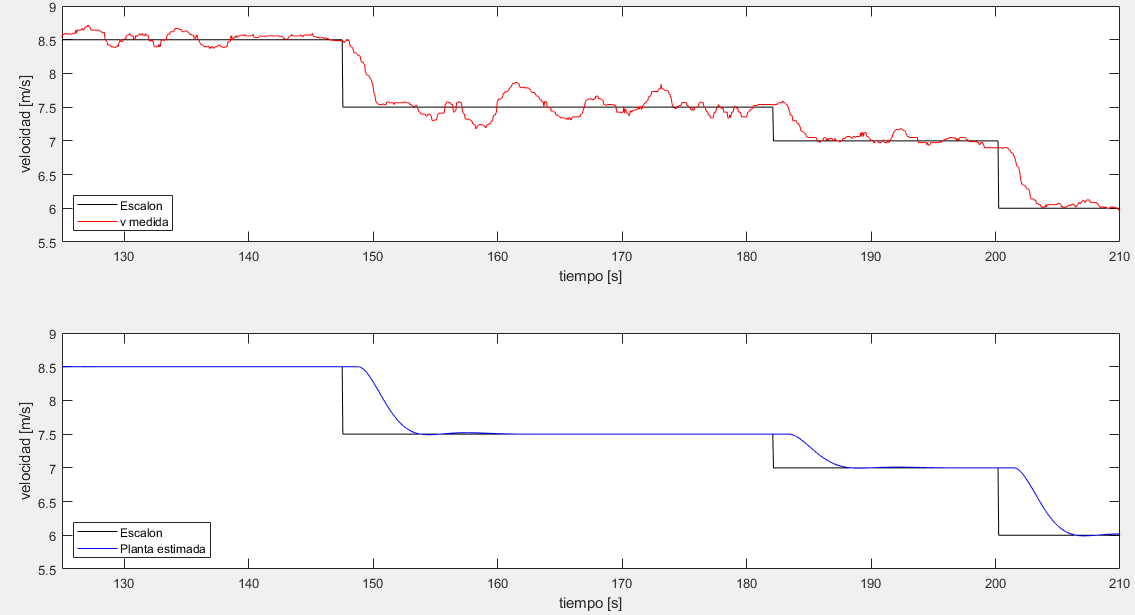
\includegraphics[scale=0.5]{Compa_Prueba7.png}
	\captionof{figure}{Datos Experimentales y Simulados para la \textit{Prueba7}}
	\label{fig:Prueba_7}
\end{figure}   
    \subsubsection{Implementación en $\mu$C}
    
    Para poder implementar en nuestro $\mu$C  el PID, se partió de la estructura interna o fórmula del controlador general discreto en el dominio Z (Ecuación \ref{PIDZ}) y se trabajó algebraicamente hasta llegar a una forma en donde aplicar la \textit{Transformada Inversa Z} no presente inconvenientes. Se utiliza esta herramienta matemática para llevar la ecuación del PID(z) al dominio del tiempo discreto.
    
     \begin{equation}
    PID(Z)\;=\;P\;+\;I.T_S.\frac1{z-1}+D.\frac1{T_S}.\frac{z-1}z \label{PIDZ}
    \end{equation}

\subsubsection{Pruebas de control}
Para observar la respuesta del control se generó perturbaciones con las compuertas laterales del túnel (Figura \ref{fig:comp}), antes utilizadas para realizar variaciones de velocidad\cite{barila1993desarrollo} cuando el laboratorio no poseía un control continuo de velocidad y se utilizaba el motor con un reóstato (Figura \ref{fig:reos}). 

\begin{figure}[H]
	\centering
	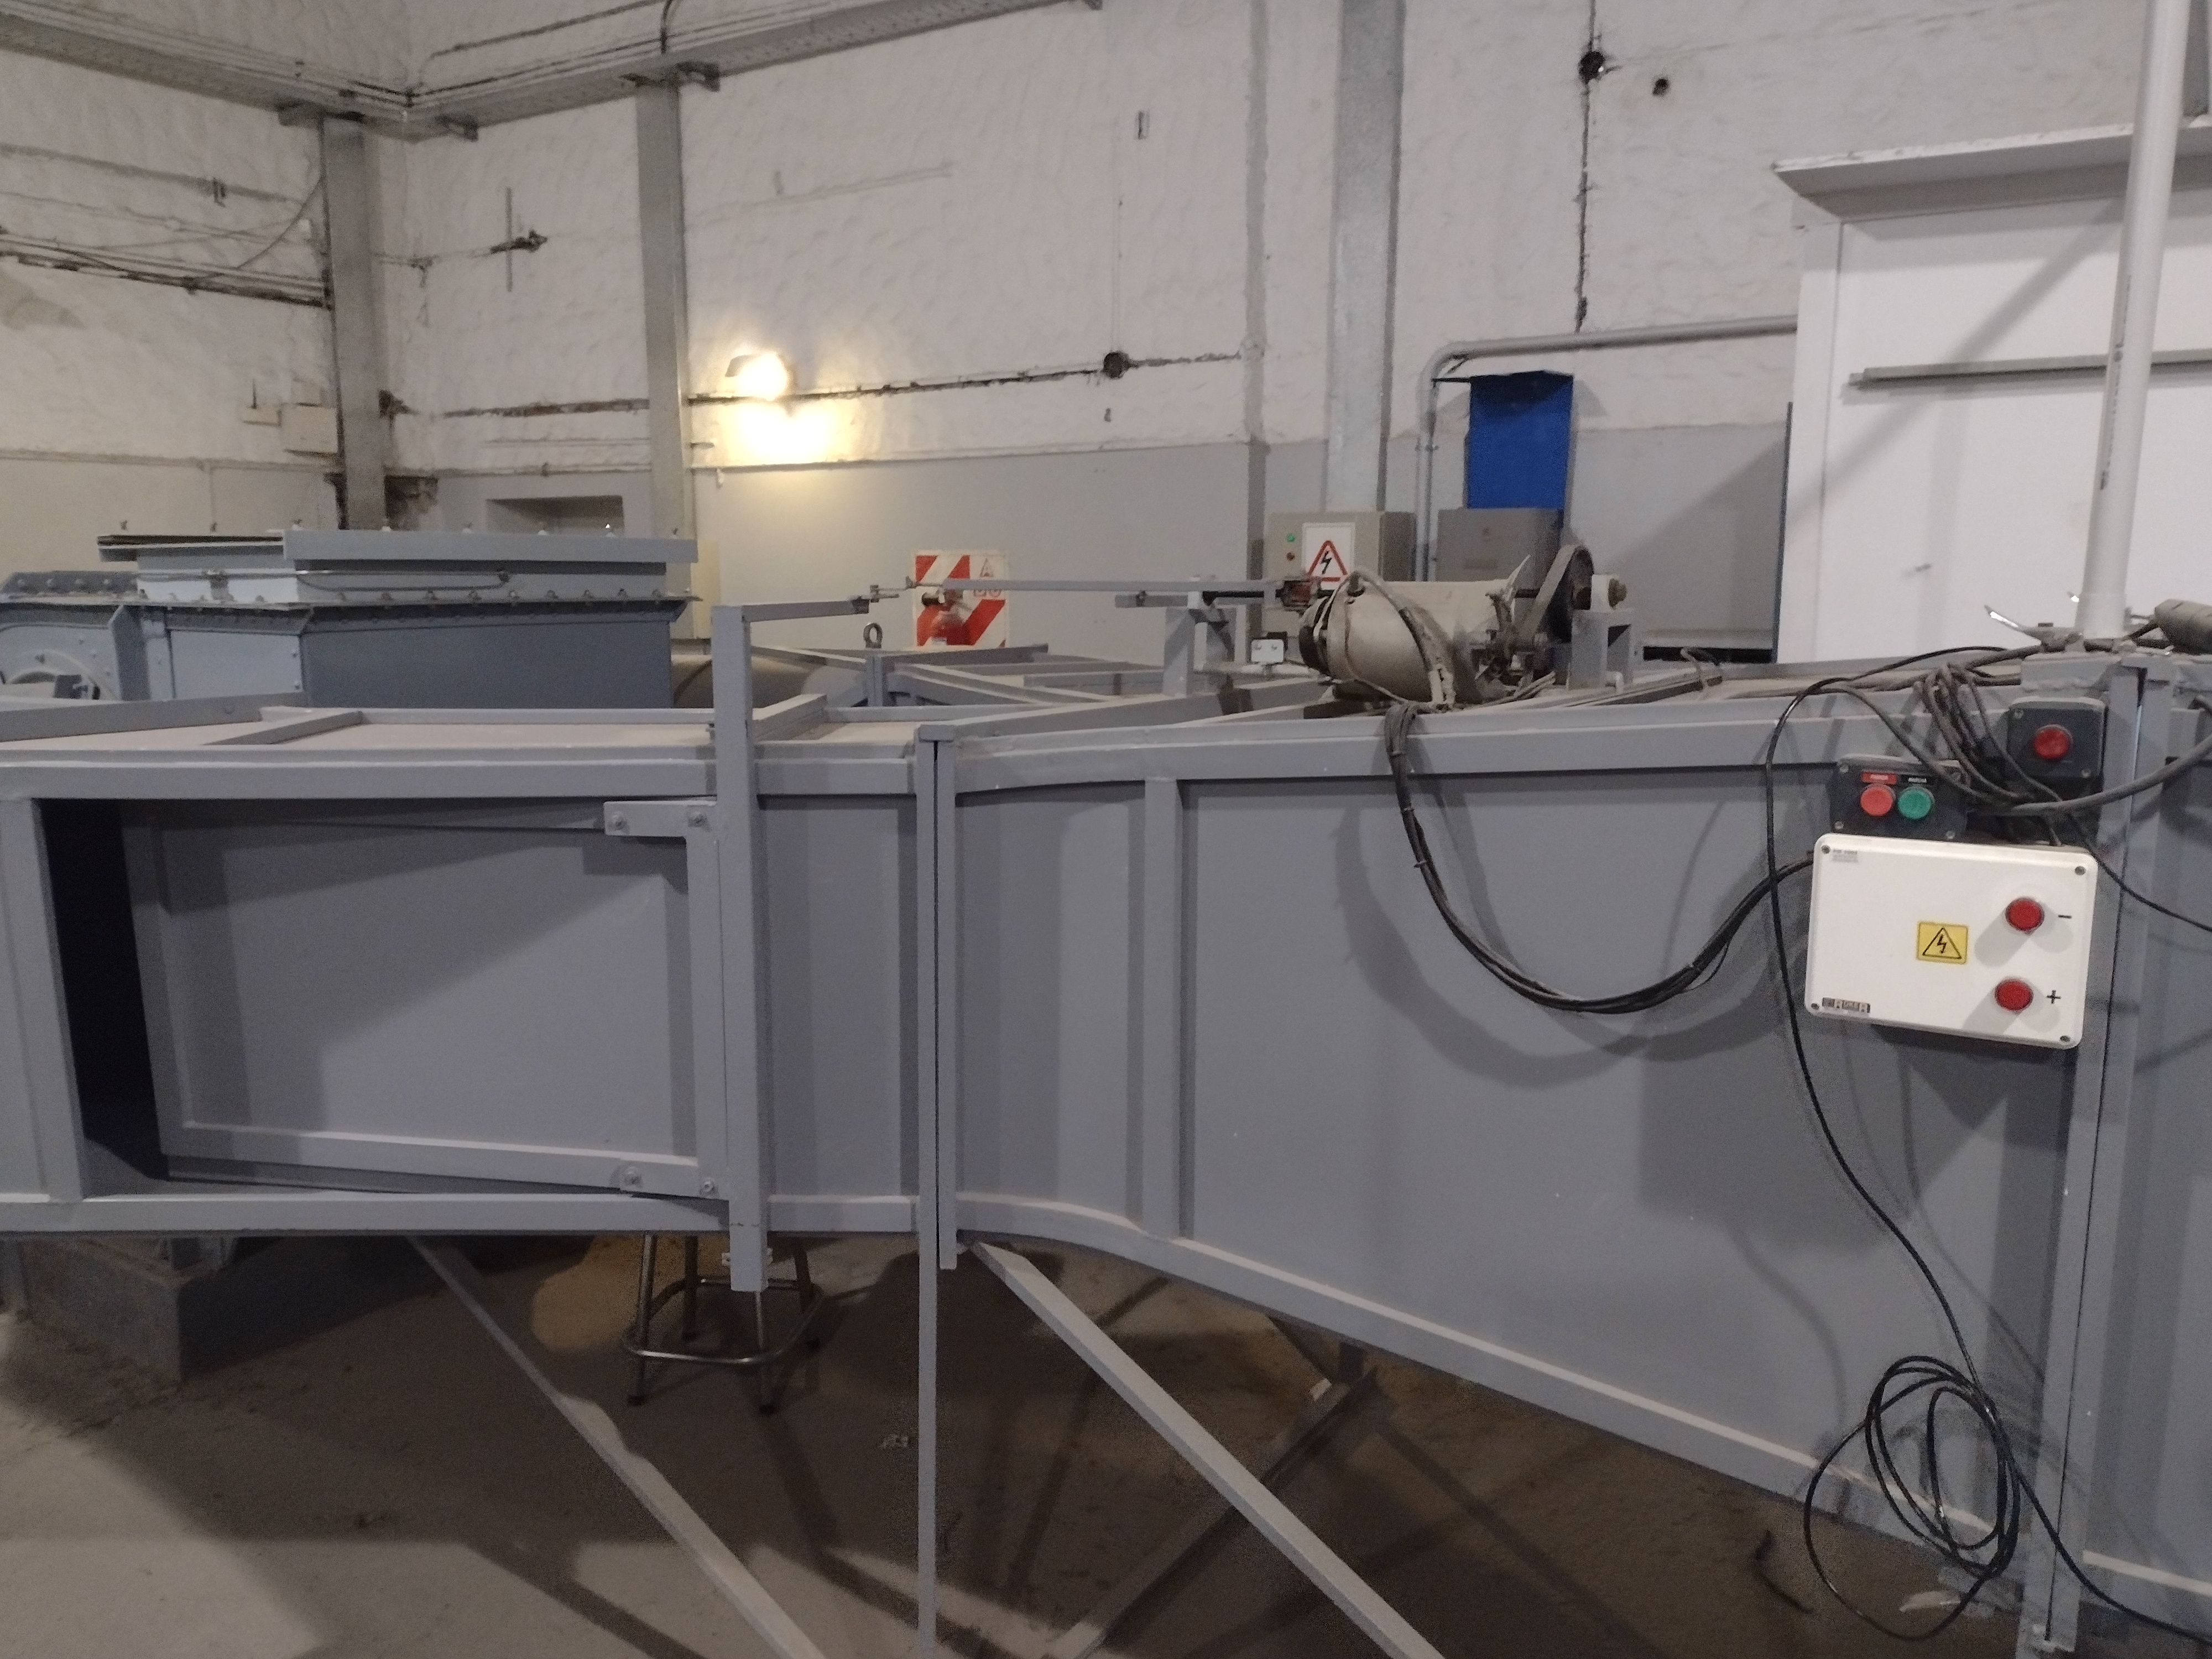
\includegraphics[scale=0.08]{comp.jpg}
	\captionof{figure}{Compuertas utilizadas como perturbaciones}
	\label{fig:comp}
\end{figure}

\begin{figure}[H]
	\centering
	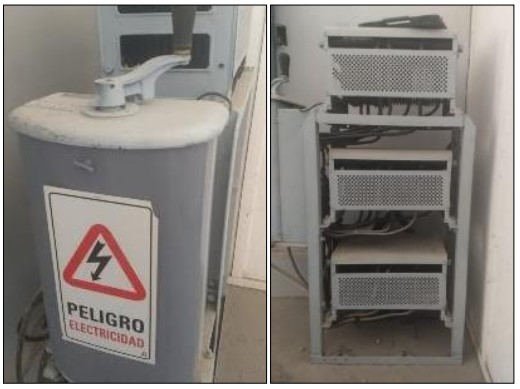
\includegraphics[scale=0.7]{reos.jpg}
	\captionof{figure}{Fotos del reóstato (izquierda) y del banco de resistencias (derecha)}
	\label{fig:reos}
\end{figure}

Para realizar estas pruebas de funcionamiento primero se encendió el túnel, se comenzó a guardar valores y se controló la velocidad del aire en 6 $m/s$, luego de unos segundos de funcionamiento se procedió a abrir las compuertas con el panel que se ve del lado derecho de la figura \ref{fig:comp}. Esta entrada de aire producía variaciones en la velocidad que el control implementado corregía según el PID utilizado. Se realizó pruebas donde se abrió y cerró las compuertas para observar estos cambios y el correcto control de velocidad (Figura \ref{fig:comp1} y \ref{fig:comp2}).


\begin{figure}[H]
	\centering
	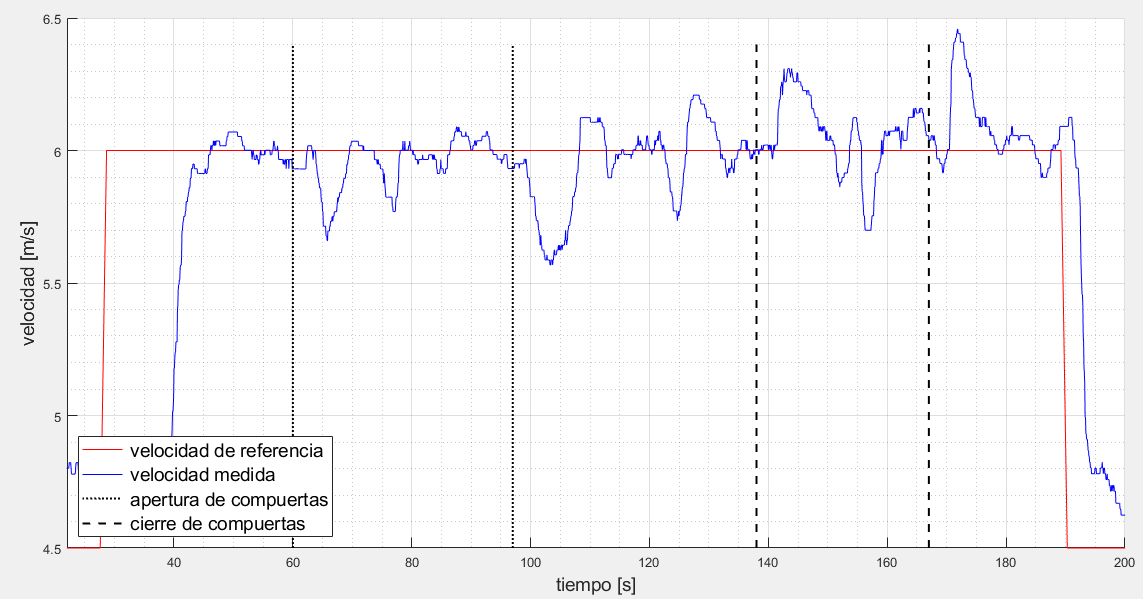
\includegraphics[scale=0.5]{compu1.png}
	\captionof{figure}{Comportamiento del sistema ante perturbaciones. Ejemplo 1.}
	\label{fig:comp1}
	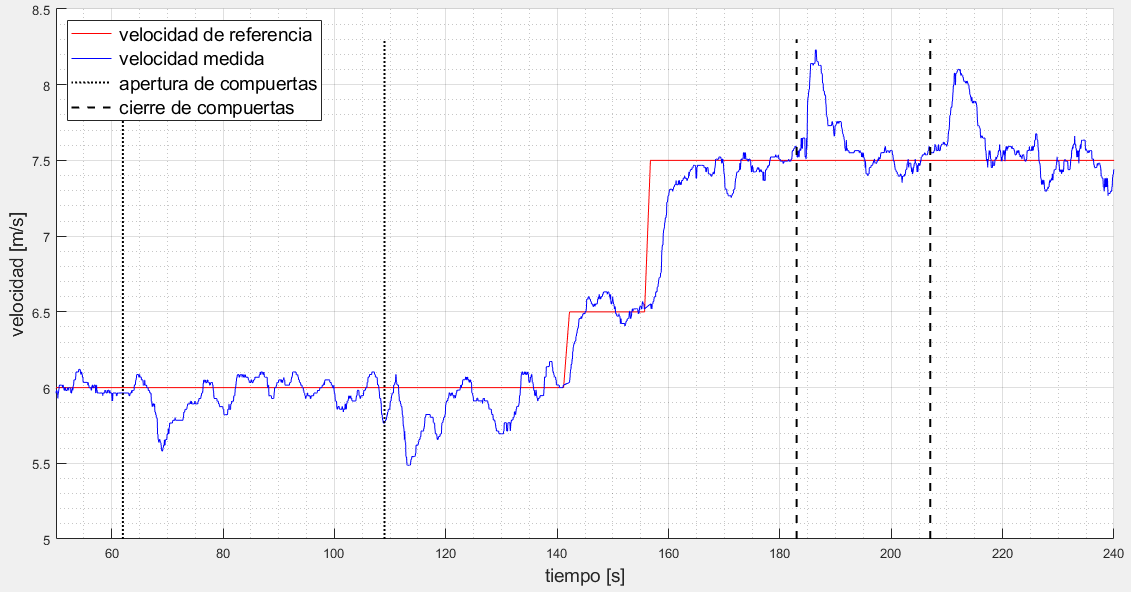
\includegraphics[scale=0.5]{comp2.png}
	\captionof{figure}{Comportamiento del sistema ante perturbaciones. Ejemplo 2.}
	\label{fig:comp2}
\end{figure}



    \newpage